\chapter{方案实现}
\label{chapter:implement}
本章重点介绍了底层感知的高性能NFV平台的具体实现。本文中,设计方案的原型的实现是在Clearwater应用框架的基础进行的。ClearWater是成熟的商用语音多媒体子系统业务框架之一。由于Clearwater在开源平台Github上开源了其所有代码,我们可以轻易的获取并在我们手中的大容量标准通用服务器上部署这项多媒体语音子系统。因此,本系统的原型实现也选择在ClearWater平台上实现。值得指出的是,虽然本系统的实现是基于ClearWater的,但是本设计中的核心设计思想和设计架构具有比较广泛的适用性,也可以适用于其他NFV业务平台。本设计使用非侵入的插入中间件方式实现,没有对业务系统有任何更改,也就是说本设计也能够扩展到其他的NFV业务中,具有一定的可扩展性。
\section{总体算法框架实现}
本设计的核心映射策略算法如算法\ref{alg:greedy}所示。根据从底层信息采用模块获取的参数信息,我们提出两种基于贪心思想的映射策略。第一种是基于服务链上任意两个相邻节点具有最大通信带宽的最大带宽策略 (GMB, Greedy Maximum Bandwidth),第二种是任意两个相邻节点具有最小通信延迟的最小延迟策略 (GML, Greedy Minimum Latency)。但带宽和延迟这两个影响因素同时可以提高整体映射策略的收益时,这两种策略可以同时被用于同一个服务链的映射生成。如果被映射的服务需要较高的通信带宽并根据其带宽来衡量其服务质量,例如数据传输服务,那么这种服务就适合使用GMB算法来生成映射结果;如果服务链的服务质量是由整体的通信延迟所决定的,那么GML便更适合这类的应用场景。当然也可以综合考虑这两个因素,使用整数线性规划的方法来求解,近期有不少针对SFC资源映射的研究就是利用这种方法来求解。
\begin{algorithm} 
	\caption{基于贪心的映射策略}  
	\label{alg:greedy}  
	\begin{algorithmic} [1]
		\State Start
		\State Backup Substrate Network State
		\For{ Function $i \in S$}
		\State Initialize: Capable Instances Set $S^{\prime} = \emptyset$
		\For{ Node $j \in D$}
		%\STATE $t_{e}= \rho_{ij} + \max(\pi_{j}, t_{i-1})$
		%\IF {$ \big( (\beta_{ij} == 1) \bigwedge (B_{j}\geq \sigma_{i})\bigwedge(t_{e} \leq t_{l}) \big)$ }
		%\STATE $S^{\prime} = S^{\prime}\uplus n$
		%\ENDIF
		\State	$P = \max(\alpha*B_{j} + \beta*L_{j})$
		\State Got L3 Cache Miss rate $\phi$ of CPU Node of $j$
		\If {$Pj  ==  \max(P)  \bigwedge Lj \leq L_{max} \bigwedge \phi < 90\% $  }
		\State $S^{\prime} = S^{\prime}\uplus j $
		\EndIf			
		\EndFor					
		\If {$S^{\prime} \equiv \emptyset$}
		\State Mapping and Scheduling Failed
		\State Reset Substrate Network Status
		\Return
		\EndIf
		\State Sort $N^{\prime}$ according to $S$	
		\State Select the top node $j^{\star}$ from $N_{\prime}$
		\State Map the function $i$ onto  $j^{\star}$
		\State Update $N_{j}$, $D_{j}$.
		\EndFor
		\State Mapping and Scheduling Completed
		\State End
	\end{algorithmic}  
\end{algorithm} 
算法\ref{alg:greedy}的具体步骤如下:当服务链请求被解析成服务链链表输出后,算法\ref{alg:greedy}将该链表$S$作为算法输入,顺序遍历该链表,针对链表中每个元素$i$,利用公式\ref{label}计算其收益函数,从待选实例中筛选出收益最大的实例并判断该实例所在计算节点的L3cache命中率,若未命中的比例超过90\%则放弃该实例选择次优收益的实例并继续比较其cache的命中率,直到有合适的实例被选中为止。通过以上的算法\ref{alg:greedy},理论上我们可以选择出相对收益最高的服务链与实例的映射链表。算法的输出结果将作为输入传入动态映射模块,该模块将根据该结果进行服务链组链操作。


\section{底层信息采样模块}
我们使用经典的内存访问测试工具Stream\footnote{https://www.cs.virginia.edu/stream/} 和Intel Memory Latency Checker\footnote{https://software.intel.com/en-us/articles/intelr-memory-latency-checker} 作为我们的采样工具,预先运行并获取所有运行时参数,作归一化处理分别后存入如下的矩阵中。在矩阵 $D$ \ref{matrix}中,元素 $D_{ij}$表示当使用第 $i$ 号访问在位于 $j$ 的资源时,所需要的性能开销。我们所使用的平台有32个物理核,即可以得到两个32x32的矩阵。所生成的信息参考矩阵被以文件的形式存储在系统硬盘上,随时供其他模块读取。
$$
M =
\begin{pmatrix}
\label{matrix}
10      & 8      & \cdots & 4      \\
9      & 10      & \cdots & 5      \\
\vdots & \vdots & \ddots & \vdots \\
4      & 3      & \cdots & 10     \\
\end{pmatrix}
$$


\section{服务链分析模块}
服务链分析模块主要负责业务接口,根据上层服务的具体需求来选择选择具体组链方式生成逻辑的服务链链表。这里我们针对Clearwater的具体业务总结了主要业务流程和所需的服务链请求。业务流程主要包括:用户注册服务,初始化拨号服务,通话服务,和通话终止。每个流程的具体流程如图\crefrange{fig:flow_register}{fig:flow_terminate}所示。
\begin{figure}[!htp]
	\centering
	\label{fig:flow_register}
	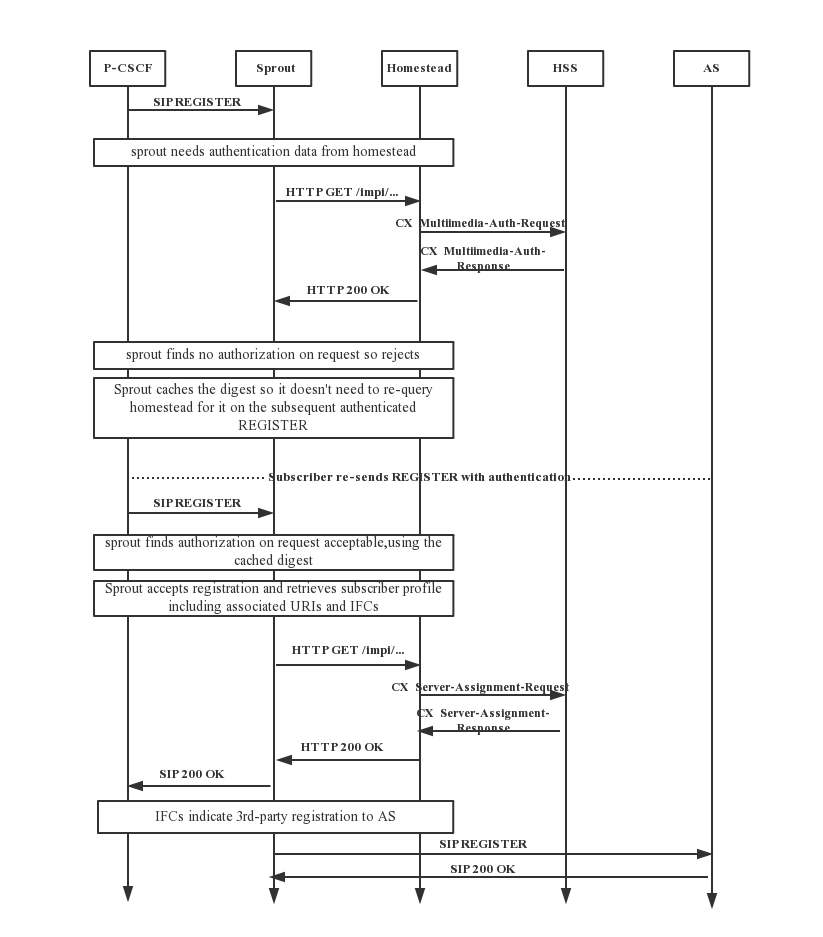
\includegraphics[width=1.0\textwidth]{clearwater/1.png}
	\bicaption[fig:flow_register]{用户注册服务流程图}{用户注册服务流程图}{Fig}{User Registration}
\end{figure}

\begin{figure}[!htp]
	\centering
	\label{fig:flow_dialog}
	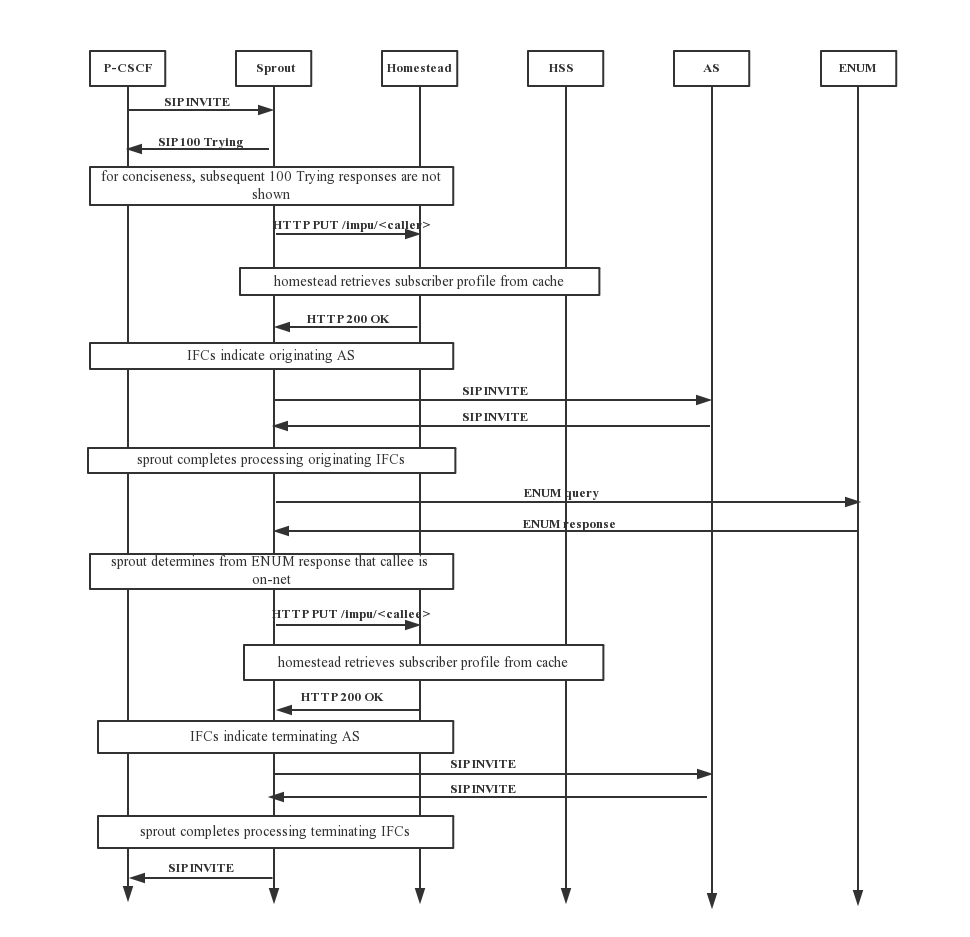
\includegraphics[width=1.0\textwidth]{clearwater/2.png}
	\bicaption[fig:flow_dialog]{初始化拨号流程}{初始化拨号流程}{Fig}{Init Dialog}
\end{figure}

\begin{figure}[!htp]
	\ContinuedFloat
	\centering
	\label{fig:flow_dialog2}
	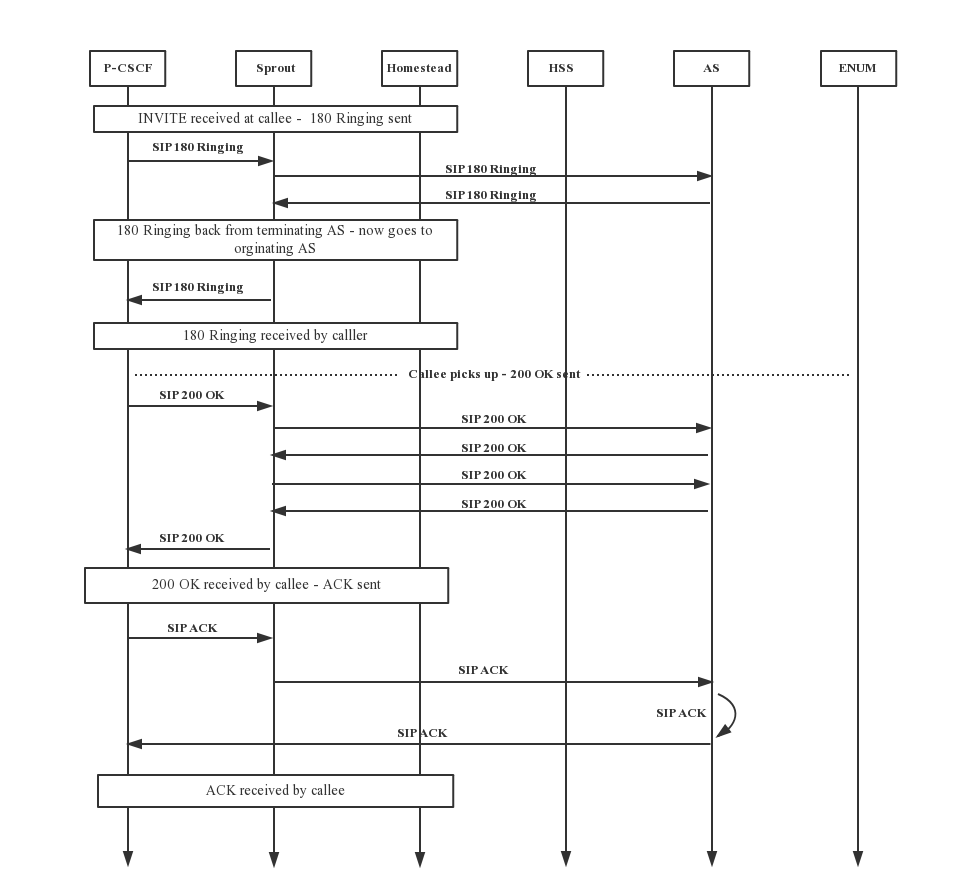
\includegraphics[width=1.0\textwidth]{clearwater/3.png}
	\bicaption[fig:flow_dialog2]{初始化拨号流程 (续)}{用户注册服务流程图}{Fig}{Init Dialog (con't)}
\end{figure}

\begin{figure}[!htp]
	\centering
	\label{fig:flow_inDialog}
	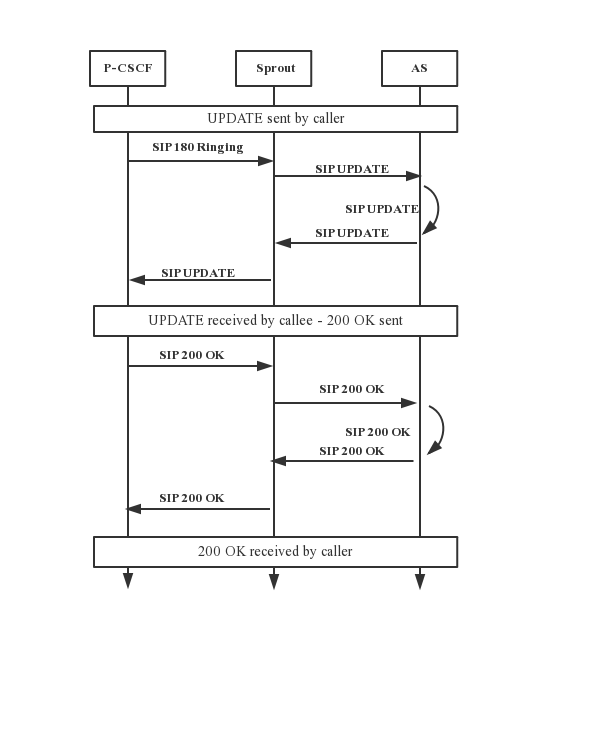
\includegraphics[width=1.0\textwidth]{clearwater/4.png}
	\bicaption[fig:flow_inDialog]{通话流程}{通话流程}{Fig}{In Dialog}
\end{figure}

\begin{figure}[!htp]
	\centering
	\label{fig:flow_terminate}
	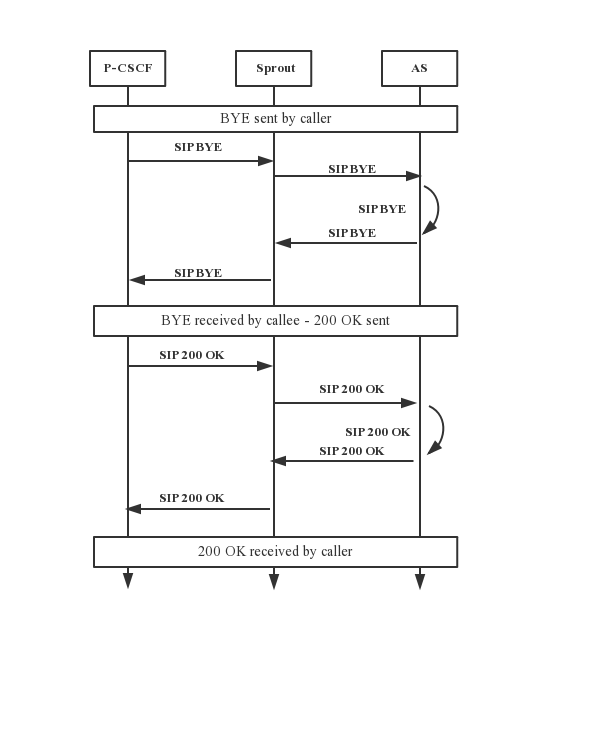
\includegraphics[width=1.0\textwidth]{clearwater/5.png}
	\bicaption[fig:flow_terminate]{通话终止流程}{通话终止流程}{Fig}{Terminate Dialog}
\end{figure}
\section{动态映射模块}
在该模块中,我们将需要根据服务链分析模块中生成的服务链组织链表通过算法\ref{alg:greedy}映射成为具体的实例链表,并根据实例链表完成服务链的组件。具体来说,我们在初始化阶段将所有的实例具体信息录入系统,包括其具体的网络功能、所分配的物理资源信息以及详细的配置参数。当具体的映射策略生成后,我们从实例列表中将实例的ip提出,通过绑定到DNS服务器的解析目录和转发列表中从而实现实例之间的物理链路组建。

\section{本章小结}
本章主要介绍了基于底层感知的高性能NFV平台的具体实现。详细介绍了平台的总体算法以及底层信息采样模块、服务链分析模块和动态映射模块的一些细节信息,给出了算法的伪代码实现以及实际服务链的流程分析。